\documentclass[11pt,a4paper]{report}
\usepackage[textwidth=37em,vmargin=30mm]{geometry}
\usepackage{calc,xunicode,amsmath,amssymb,paralist,enumitem,tabu,booktabs,datetime2,xeCJK,xeCJKfntef,listings}
\usepackage{tocloft,fancyhdr,tcolorbox,xcolor,graphicx,eso-pic,xltxtra,xelatexemoji}

\newcommand{\envyear}[0]{2025}
\newcommand{\envdatestr}[0]{2025-05-24}
\newcommand{\envfinaldir}[0]{webdb/2025/20250524/final}

\usepackage[hidelinks]{hyperref}
\hypersetup{
    colorlinks=false,
    pdfpagemode=FullScreen,
    pdftitle={Web Digest - \envdatestr}
}

\setlength{\cftbeforechapskip}{10pt}
\renewcommand{\cftchapfont}{\rmfamily\bfseries\large\raggedright}
\setlength{\cftbeforesecskip}{2pt}
\renewcommand{\cftsecfont}{\sffamily\small\raggedright}

\setdefaultleftmargin{2em}{2em}{1em}{1em}{1em}{1em}

\usepackage{xeCJK,xeCJKfntef}
\xeCJKsetup{PunctStyle=plain,RubberPunctSkip=false,CJKglue=\strut\hskip 0pt plus 0.1em minus 0.05em,CJKecglue=\strut\hskip 0.22em plus 0.2em}
\XeTeXlinebreaklocale "zh"
\XeTeXlinebreakskip = 0pt


\setmainfont{Brygada 1918}
\setromanfont{Brygada 1918}
\setsansfont{IBM Plex Sans}
\setmonofont{JetBrains Mono NL}
\setCJKmainfont{Noto Serif CJK SC}
\setCJKromanfont{Noto Serif CJK SC}
\setCJKsansfont{Noto Sans CJK SC}
\setCJKmonofont{Noto Sans CJK SC}

\setlength{\parindent}{0pt}
\setlength{\parskip}{8pt}
\linespread{1.15}

\lstset{
	basicstyle=\ttfamily\footnotesize,
	numbersep=5pt,
	backgroundcolor=\color{black!5},
	showspaces=false,
	showstringspaces=false,
	showtabs=false,
	tabsize=2,
	captionpos=b,
	breaklines=true,
	breakatwhitespace=true,
	breakautoindent=true,
	linewidth=\textwidth
}






\newcommand{\coverpic}[2]{
    % argv: itemurl, authorname
    Cover photo by #2~~(\href{#1}{#1})
}
\newcommand{\makeheader}[0]{
    \begin{titlepage}
        % \newgeometry{hmargin=15mm,tmargin=21mm,bmargin=12mm}
        \begin{center}
            
            \rmfamily\scshape
            \fontspec{BaskervilleF}
            \fontspec{Old Standard}
            \fontsize{59pt}{70pt}\selectfont
            WEB\hfill DIGEST
            
            \vfill
            % \vskip 30pt
            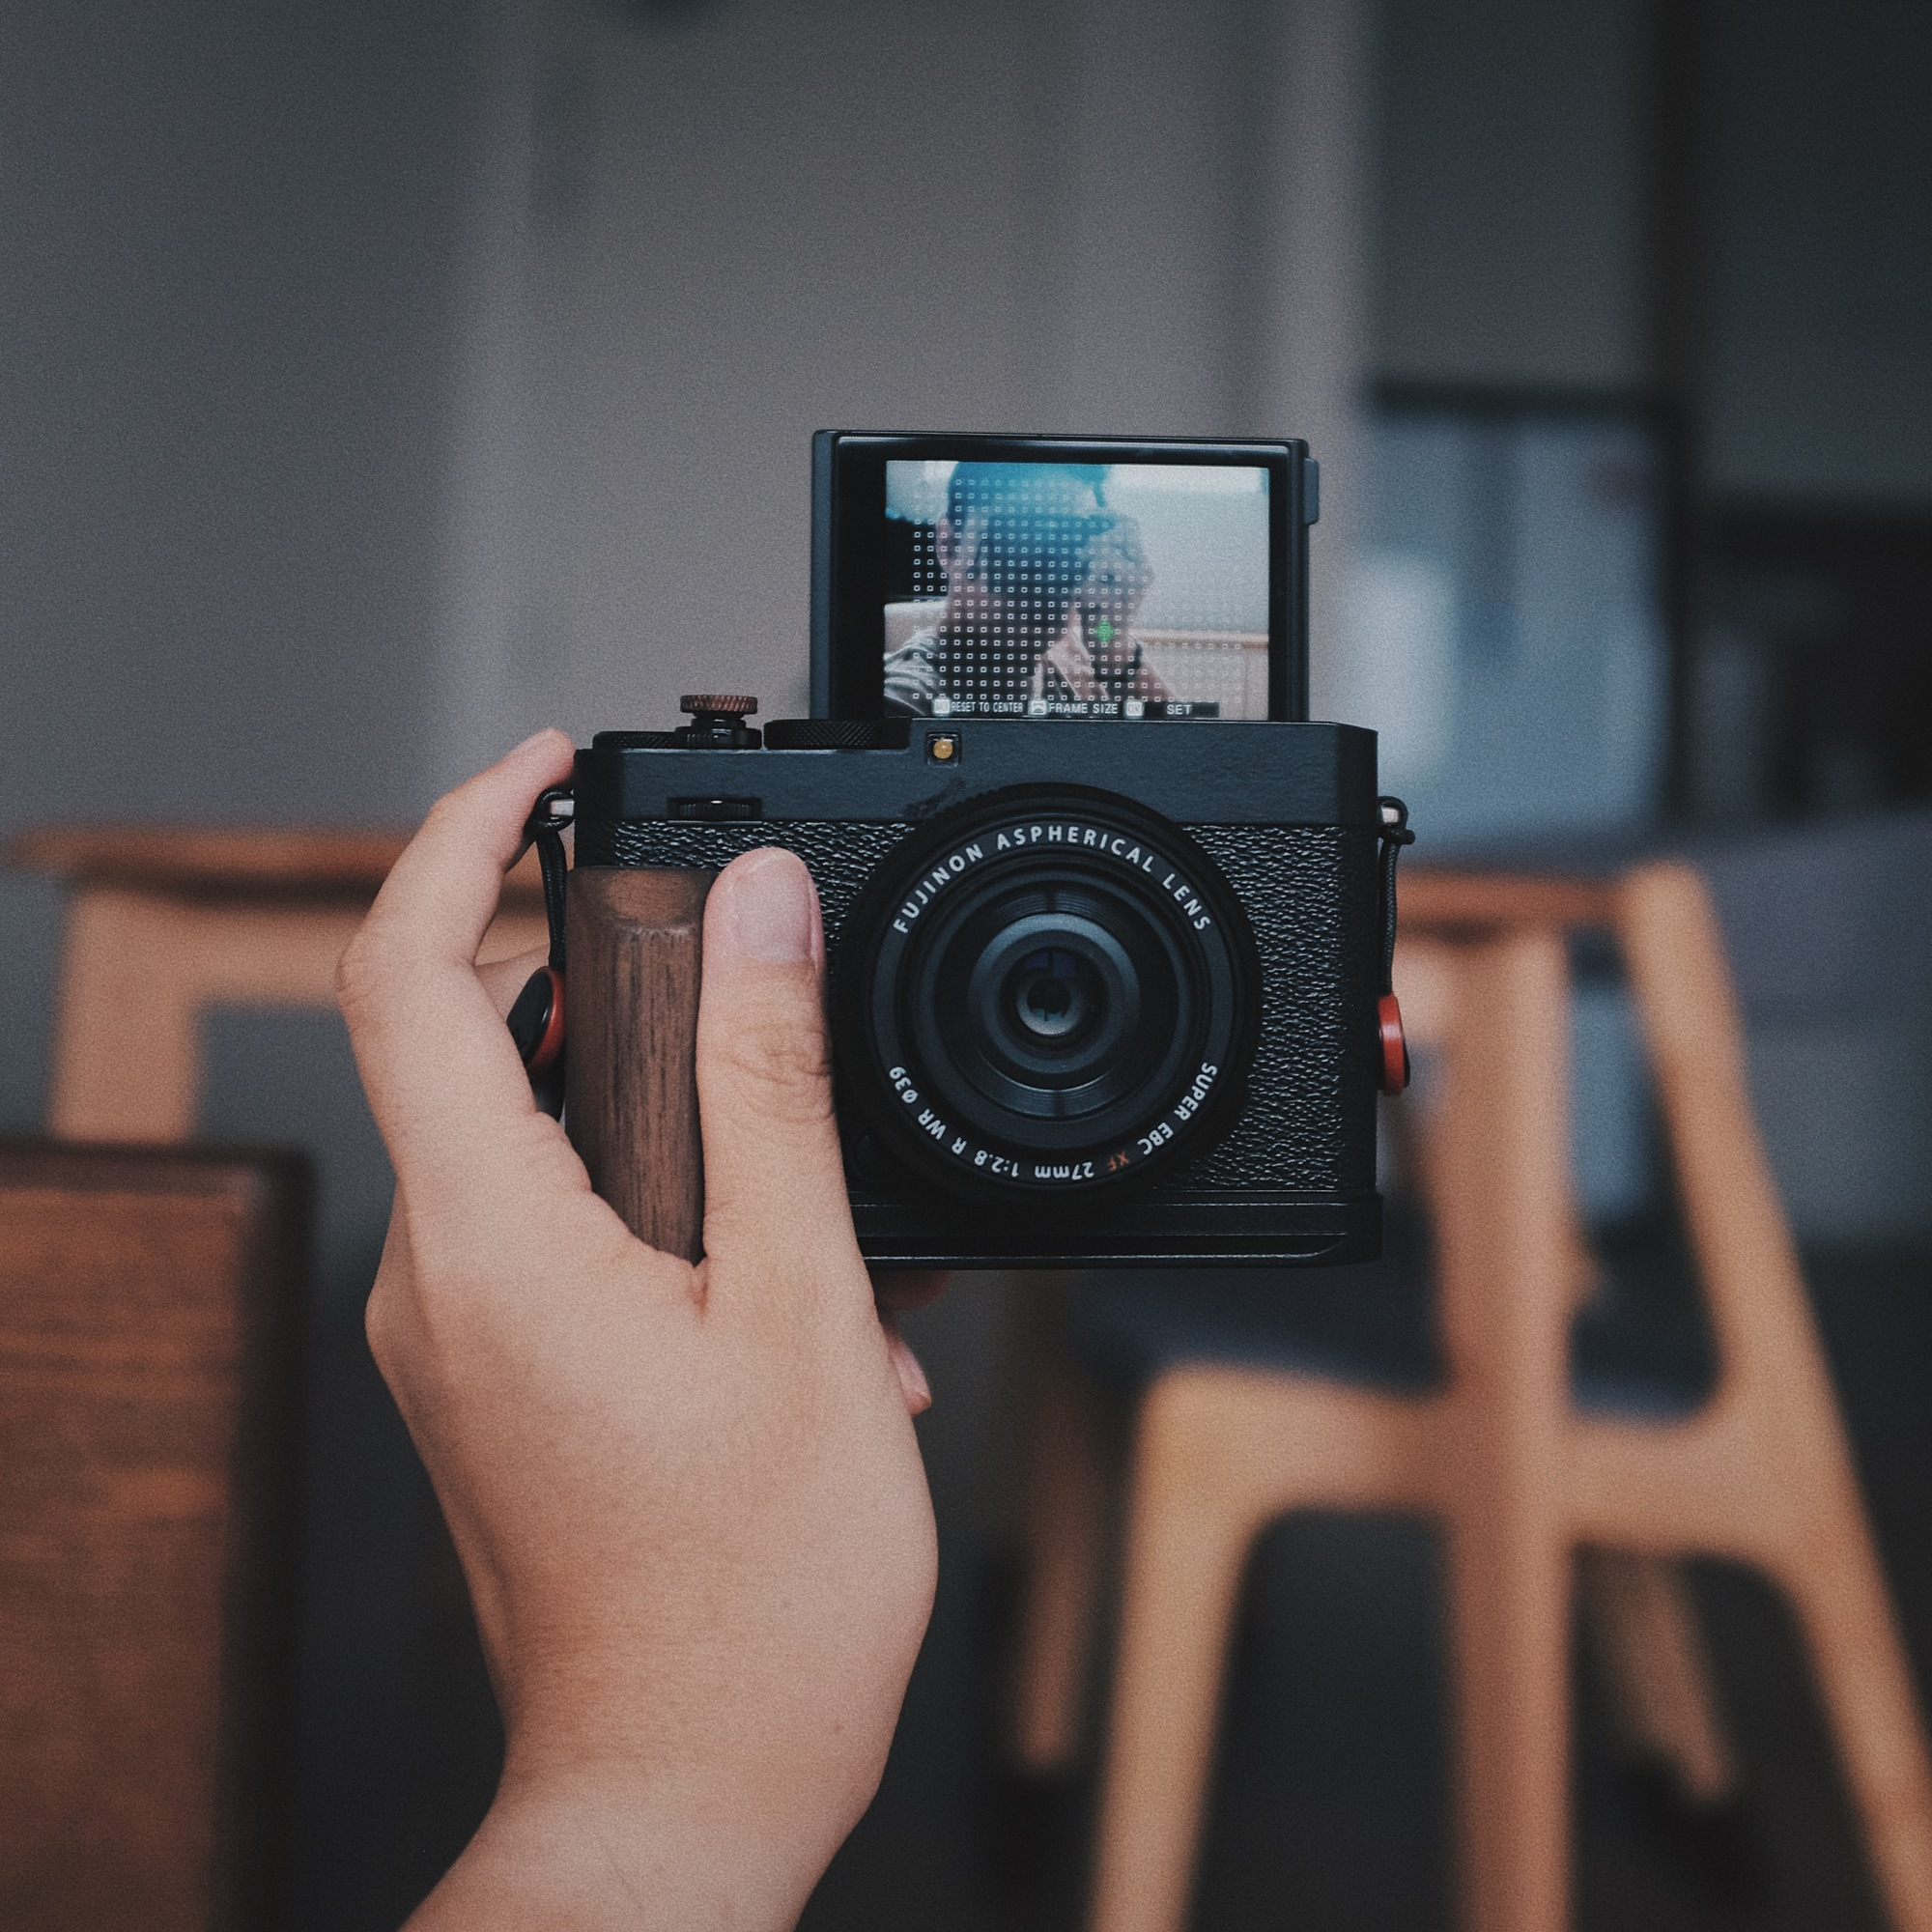
\includegraphics[width=\linewidth]{\envfinaldir/coverpic-prod.jpg}\par
            % \vskip 30pt
            \vfill

            \normalsize\rmfamily\scshape
            \copyright{} The Web Digest Project \hfill\large \envdatestr
        \end{center}
    \end{titlepage}
    % \restoregeometry
}
\newcommand{\simplehref}[1]{%
    \textcolor{blue!80!green}{\href{#1}{#1}}%
}
\renewcommand{\contentsname}{\center\Huge\sffamily\bfseries Contents\par\vskip 20pt}
\newcounter{ipartcounter}
\setcounter{ipartcounter}{0}
\newcommand{\ipart}[1]{
    % \vskip 20pt
    \clearpage
    \stepcounter{ipartcounter}
    \phantomsection
    \addcontentsline{toc}{chapter}{#1}
    % \begin{center}
    %     \Huge
    %     \sffamily\bfseries
    %     #1
    % \end{center}
    % \vskip 20pt plus 7pt
}
\newcounter{ichaptercounter}
\setcounter{ichaptercounter}{0}
\newcommand{\ichapter}[1]{
    % \vskip 20pt
    \clearpage
    \stepcounter{ichaptercounter}
    \phantomsection
    \addcontentsline{toc}{section}{\numberline{\arabic{ichaptercounter}}#1}
    \begin{center}
        \Huge
        \sffamily\bfseries
        #1
    \end{center}
    \vskip 20pt plus 7pt
}
\newcommand{\entrytitlefont}[1]{\subsection*{\raggedright\Large\sffamily\bfseries#1}}
\newcommand{\entryitemGeneric}[2]{
    % argv: title, url
    \parbox{\linewidth}{
        \entrytitlefont{#1}\par\vskip 5pt
        \footnotesize\ttfamily\mdseries
        \simplehref{#2}
    }\vskip 11pt plus 11pt minus 1pt
}
\newcommand{\entryitemGithub}[3]{
    % argv: title, url, desc
    \parbox{\linewidth}{
        \entrytitlefont{#1}\par\vskip 5pt
        \footnotesize\ttfamily\mdseries
        \simplehref{#2}\par\vskip 5pt
        \small\rmfamily\mdseries#3
    }\vskip 11pt plus 11pt minus 1pt
}
\newcommand{\entryitemAp}[3]{
    % argv: title, url, desc
    \parbox{\linewidth}{
        \entrytitlefont{#1}\par\vskip 5pt
        \footnotesize\ttfamily\mdseries
        \simplehref{#2}\par\vskip 5pt
        \small\rmfamily\mdseries#3
    }\vskip 11pt plus 11pt minus 1pt
}
\newcommand{\entryitemHackernews}[3]{
    % argv: title, hnurl, rawurl
    % \parbox{\linewidth}{
    %     \entrytitlefont{#1}\par\vskip 5pt
    %     \footnotesize\ttfamily\mdseries
    %     \simplehref{#3}\par
    %     \textcolor{black!50}{\href{#2}{#2}}
    % }\vskip 11pt plus 11pt minus 1pt
    \begin{minipage}{\linewidth}
            \entrytitlefont{#1}\par\vskip 5pt
            \footnotesize\ttfamily\mdseries
            \simplehref{#3}\par
            \textcolor{black!50}{\href{#2}{#2}}
    \end{minipage}\par\vskip 11pt plus 11pt minus 1pt
}







\begin{document}

\makeheader

\tableofcontents\clearpage




\ipart{Developers}
\ichapter{Hacker News}
\entryitemTwoLinks{Show HN: hcker.news – an ergonomic, timeline-based Hacker News front page}{https://news.ycombinator.com/item?id=44075353}{https://hcker.news}

\entryitemTwoLinks{How to live on \$432 a month in America}{https://news.ycombinator.com/item?id=44074340}{https://shagbark.substack.com/p/how-to-live-on-432-a-month-in-america}

\entryitemTwoLinks{Find Your People}{https://news.ycombinator.com/item?id=44074017}{https://foundersatwork.posthaven.com/find-your-people}

\entryitemTwoLinks{MCP is the coming of Web 2.0 2.0}{https://news.ycombinator.com/item?id=44073785}{https://www.anildash.com//2025/05/20/mcp-web20-20/}

\entryitemTwoLinks{Postgres IDE in VS Code}{https://news.ycombinator.com/item?id=44073588}{https://techcommunity.microsoft.com/blog/adforpostgresql/announcing-a-new-ide-for-postgresql-in-vs-code-from-microsoft/4414648}

\entryitemTwoLinks{Caesar's Last Breath}{https://news.ycombinator.com/item?id=44073185}{https://charliesabino.com/caesars-last-breath/}

\entryitemTwoLinks{How I ended up flying for Yemen's national airline – and survived}{https://news.ycombinator.com/item?id=44072971}{https://www.pprune.org/terms-endearment/653181-yemenia-expat-contract-full-info.html}

\entryitemTwoLinks{Remembering Alasdair MacIntyre}{https://news.ycombinator.com/item?id=44071900}{https://www.wordonfire.org/articles/remembering-alasdair-macintyre-1929-2025/}

\entryitemTwoLinks{Why I no longer have an old-school cert on my HTTPS site}{https://news.ycombinator.com/item?id=44071690}{https://rachelbythebay.com/w/2025/05/22/ssl/}

\entryitemTwoLinks{Writing A Job Runner (In Elixir) (Again) (10 years later)}{https://news.ycombinator.com/item?id=44071610}{https://github.com/notactuallytreyanastasio/genstage\_tutorial\_2025/blob/main/README.md}

\entryitemTwoLinks{OpenAI: Scaling PostgreSQL to the Next Level}{https://news.ycombinator.com/item?id=44071418}{https://www.pixelstech.net/article/1747708863-openai\%3a-scaling-postgresql-to-the-next-level}

\entryitemTwoLinks{KumoRFM: A Foundation Model for In-Context Learning on Relational Data}{https://news.ycombinator.com/item?id=44070532}{https://kumo.ai/company/news/kumo-relational-foundation-model/}

\entryitemTwoLinks{John Carmack talk at Upper Bound 2025}{https://news.ycombinator.com/item?id=44070042}{https://twitter.com/ID\_AA\_Carmack/status/1925710474366034326}

\entryitemTwoLinks{The copilot delusion}{https://news.ycombinator.com/item?id=44068525}{https://deplet.ing/the-copilot-delusion/}

\entryitemTwoLinks{The Future of Flatpak}{https://news.ycombinator.com/item?id=44068400}{https://lwn.net/Articles/1020571/}

\entryitemTwoLinks{Sketchy Calendar}{https://news.ycombinator.com/item?id=44068204}{https://www.inkandswitch.com/ink/notes/sketchy-calendar/}

\entryitemTwoLinks{32 bits that changed microprocessor design}{https://news.ycombinator.com/item?id=44068197}{https://spectrum.ieee.org/bellmac-32-ieee-milestone}

\entryitemTwoLinks{Show HN: Defuddle, an HTML-to-Markdown alternative to Readability}{https://news.ycombinator.com/item?id=44067409}{https://github.com/kepano/defuddle}

\entryitemTwoLinks{1,145 pull requests per day}{https://news.ycombinator.com/item?id=44065680}{https://saile.it/1145-pull-requests-per-day/}

\entryitemTwoLinks{Does Earth have two high-tide bulges on opposite sides? (2014)}{https://news.ycombinator.com/item?id=44065458}{http://physics.stackexchange.com/questions/121830/does-earth-really-have-two-high-tide-bulges-on-opposite-sides}\ichapter{Phoronix}
\entryitemGeneric{\hskip 0pt{}Microsoft Lands 62k Lines Of Code Patch In Mesa: Adds New "MFT" Gallium3D Frontend}{https://www.phoronix.com/news/Microsoft-Lands-MFT-Gallium3D}

\entryitemGeneric{\hskip 0pt{}Linux 6.15 Brings Many Features For Intel \& AMD Hardware}{https://www.phoronix.com/news/Linux-6.15-Features-Reminder}

\entryitemGeneric{\hskip 0pt{}GNOME Help \& Documentation Are In Need Of Help}{https://www.phoronix.com/news/GNOME-Help-Needs-Help}

\entryitemGeneric{\hskip 0pt{}Benchmarks: OpenCL Kernel Latency ~76x Lower For Intel Lunar Lake With Updated Compute Runtime}{https://www.phoronix.com/review/intel-lunar-lake-compute-ulls}

\entryitemGeneric{\hskip 0pt{}GCC 14.3 Compiler Released With 200+ Bug Fixes}{https://www.phoronix.com/news/GCC-14.3-Released}

\entryitemGeneric{\hskip 0pt{}Linux 6.15 Sees Last Minute Power Savings Fix For Intel Arrow Lake U/H}{https://www.phoronix.com/news/Linux-6.15-Fix-ARL-U-H-s2idle}

\entryitemGeneric{\hskip 0pt{}Mesa Will Stop Building Gallium-XA By Default}{https://www.phoronix.com/news/Mesa-Stop-Building-XA}

\entryitemGeneric{\hskip 0pt{}AMD Previews Mysterious Linux Runtime Stack For Ryzen AI NPUs}{https://www.phoronix.com/news/AMD-Linux-RT-Preview-Ryzen-AI}

\entryitemGeneric{\hskip 0pt{}Wayland 1.24 Release Candidate Brings Few Changes}{https://www.phoronix.com/news/Wayland-1.24-RC1}\ichapter{Dribbble}
\entryitemGeneric{\hskip 0pt{}Meditation App Branding Concept}{https://dribbble.com/shots/26057810-Meditation-App-Branding-Concept}

\entryitemGeneric{\hskip 0pt{}Landing Page for an AI-Powered Design System}{https://dribbble.com/shots/26057663-Landing-Page-for-an-AI-Powered-Design-System}

\entryitemGeneric{\hskip 0pt{}Smart Home App}{https://dribbble.com/shots/26056748-Smart-Home-App}

\entryitemGeneric{\hskip 0pt{}Medic H - Logo Design}{https://dribbble.com/shots/26057472-Medic-H-Logo-Design}

\entryitemGeneric{\hskip 0pt{}Sellin dashboard}{https://dribbble.com/shots/26037015-Sellin-dashboard}

\entryitemGeneric{\hskip 0pt{}Illustration}{https://dribbble.com/shots/26052539-Illustration}

\entryitemGeneric{\hskip 0pt{}Playground web interaction}{https://dribbble.com/shots/26048246-Playground-web-interaction}

\entryitemGeneric{\hskip 0pt{}Travel Startup Branding for Holidu: visual identity brand design}{https://dribbble.com/shots/25983747-Travel-Startup-Branding-for-Holidu-visual-identity-brand-design}

\entryitemGeneric{\hskip 0pt{}Onday - Logo Design}{https://dribbble.com/shots/26053436-Onday-Logo-Design}

\entryitemGeneric{\hskip 0pt{}Burger Time!}{https://dribbble.com/shots/26053795-Burger-Time}

\entryitemGeneric{\hskip 0pt{}DICH™ Fashion Vol.2}{https://dribbble.com/shots/26046875-DICH-Fashion-Vol-2}

\entryitemGeneric{\hskip 0pt{}L'Renee \& Associates logo}{https://dribbble.com/shots/26047943-L-Renee-Associates-logo}

\entryitemGeneric{\hskip 0pt{}Magus Logo Design}{https://dribbble.com/shots/26048055-Magus-Logo-Design}

\entryitemGeneric{\hskip 0pt{}Account Dropdown}{https://dribbble.com/shots/26047665-Account-Dropdown}

\entryitemGeneric{\hskip 0pt{}Chromix – Logo Design // For Sale}{https://dribbble.com/shots/26048061-Chromix-Logo-Design-For-Sale}

\entryitemGeneric{\hskip 0pt{}F}{https://dribbble.com/shots/26041370-F}

\entryitemGeneric{\hskip 0pt{}Howdy from a happy hermit!}{https://dribbble.com/shots/26043217-Howdy-from-a-happy-hermit}

\entryitemGeneric{\hskip 0pt{}Dark or Light?}{https://dribbble.com/shots/26042325-Dark-or-Light}

\entryitemGeneric{\hskip 0pt{}Mackerel}{https://dribbble.com/shots/26043994-Mackerel}

\entryitemGeneric{\hskip 0pt{}Evergreen}{https://dribbble.com/shots/26042187-Evergreen}

\entryitemGeneric{\hskip 0pt{}Planto}{https://dribbble.com/shots/26044620-Planto}

\entryitemGeneric{\hskip 0pt{}Ebay Rebranding Concept}{https://dribbble.com/shots/26039712-Ebay-Rebranding-Concept}

\entryitemGeneric{\hskip 0pt{}QueenClub Logo Design}{https://dribbble.com/shots/26042947-QueenClub-Logo-Design}

\entryitemGeneric{\hskip 0pt{}Finance Landing Page Design}{https://dribbble.com/shots/26037973-Finance-Landing-Page-Design}


\ipart{Developers~~~~(zh-Hans)}
\ichapter{Solidot}
\entryitemGeneric{\hskip 0pt{}天文学家首次观测到 110 亿光年外遥远星系的碰撞}{https://www.solidot.org/story?sid=81377}

\entryitemGeneric{\hskip 0pt{}Flatpak 的未来面临不确定性}{https://www.solidot.org/story?sid=81376}

\entryitemGeneric{\hskip 0pt{}微塑料悄悄从土壤扩散到沙拉再到人类}{https://www.solidot.org/story?sid=81375}

\entryitemGeneric{\hskip 0pt{}新隐形眼镜实现近红外色彩图像视觉}{https://www.solidot.org/story?sid=81374}

\entryitemGeneric{\hskip 0pt{}微软为记事本加入文本生成功能}{https://www.solidot.org/story?sid=81373}

\entryitemGeneric{\hskip 0pt{}研究发现虎妈式教育能提高青少年认知能力但会损害情感发展}{https://www.solidot.org/story?sid=81372}

\entryitemGeneric{\hskip 0pt{}养狗重新定义家庭和育儿}{https://www.solidot.org/story?sid=81371}

\entryitemGeneric{\hskip 0pt{}俄罗斯将要求莫斯科所有外国人安装位置跟踪应用}{https://www.solidot.org/story?sid=81370}

\entryitemGeneric{\hskip 0pt{}大型树懒因人类活动而灭绝}{https://www.solidot.org/story?sid=81369}

\entryitemGeneric{\hskip 0pt{}Mozilla 宣布 7 月 8 日关闭 Pocket}{https://www.solidot.org/story?sid=81368}

\entryitemGeneric{\hskip 0pt{}健美先生有高死亡风险}{https://www.solidot.org/story?sid=81367}

\entryitemGeneric{\hskip 0pt{}Signal 在默认下不能被 Recall}{https://www.solidot.org/story?sid=81366}

\entryitemGeneric{\hskip 0pt{}AI 用电量到 2028 年将占到美国家庭用电量的 22\%}{https://www.solidot.org/story?sid=81365}

\entryitemGeneric{\hskip 0pt{}调查显示马斯克旗下品牌声誉急剧下跌}{https://www.solidot.org/story?sid=81364}

\entryitemGeneric{\hskip 0pt{}微软内部邮件系统屏蔽``巴勒斯坦''}{https://www.solidot.org/story?sid=81363}

\entryitemGeneric{\hskip 0pt{}Windows 11 将提供类似苹果 App Continuity 的跨设备恢复功能}{https://www.solidot.org/story?sid=81362}

\entryitemGeneric{\hskip 0pt{}OpenAI 以 65 亿美元收购 Jony Ive 创办的 io 公司}{https://www.solidot.org/story?sid=81361}

\entryitemGeneric{\hskip 0pt{}微软称全世界有 39.4 万台 Windows 电脑感染了 Lumma 恶意程序}{https://www.solidot.org/story?sid=81360}

\entryitemGeneric{\hskip 0pt{}Google 搜索关键词历史抓获 2020 年丹佛致命纵火案凶手}{https://www.solidot.org/story?sid=81359}

\entryitemGeneric{\hskip 0pt{}巴西研究人员抓取 20 亿条 Discord 消息公开发布}{https://www.solidot.org/story?sid=81358}\ichapter{V2EX}
\entryitemGeneric{\hskip 0pt{}[宽带症候群] 个人免翻墙跨境流量 比 横琴宽带 门槛更低}{https://www.v2ex.com/t/1133954}

\entryitemGeneric{\hskip 0pt{}[远程工作] [远程] [金融] [高级全栈 AI 工程师]}{https://www.v2ex.com/t/1133953}

\entryitemGeneric{\hskip 0pt{}[职场话题] 大二计算机,求指路}{https://www.v2ex.com/t/1133952}

\entryitemGeneric{\hskip 0pt{}[旅行] 暑期法意瑞自驾 12 天,求路线推荐}{https://www.v2ex.com/t/1133950}

\entryitemGeneric{\hskip 0pt{}[程序员] 请教各位大佬一个封装多 Agent 的一个问题}{https://www.v2ex.com/t/1133949}

\entryitemGeneric{\hskip 0pt{}[Apple] iOS 的 Safari 体验已经如此拉跨了?}{https://www.v2ex.com/t/1133948}

\entryitemGeneric{\hskip 0pt{}[天黑以后] 20250523 午夜俱乐部}{https://www.v2ex.com/t/1133947}

\entryitemGeneric{\hskip 0pt{}[生活] 询问一下各位朋友的体温,我发觉我自身体温有时候总是有点高,但是低于 37.2,属于正常区间,好多年了(有些困扰我}{https://www.v2ex.com/t/1133946}

\entryitemGeneric{\hskip 0pt{}[Python] [真·跨平台] Python 打包新思路}{https://www.v2ex.com/t/1133945}

\entryitemGeneric{\hskip 0pt{}[程序员] Claude Sonnet 4 为什么这么喜欢写代码}{https://www.v2ex.com/t/1133944}

\entryitemGeneric{\hskip 0pt{}[Android] 三星 S24+ 更新 One UI 7.0 后耗电和发热加剧,一天一充变两充}{https://www.v2ex.com/t/1133943}

\entryitemGeneric{\hskip 0pt{}[OpenAI] claude referral 码,自取}{https://www.v2ex.com/t/1133942}

\entryitemGeneric{\hskip 0pt{}[宽带症候群] 还有人在用广州电信 199 优惠 60 的融合套餐吗}{https://www.v2ex.com/t/1133941}

\entryitemGeneric{\hskip 0pt{}[问与答] 小米微博被篡改的二维码地址是什么?}{https://www.v2ex.com/t/1133940}

\entryitemGeneric{\hskip 0pt{}[随想] "自研"其实是一个极其模糊的概念}{https://www.v2ex.com/t/1133939}

\entryitemGeneric{\hskip 0pt{}[分享创造] Proof of Awesome - 挖人矿的区块链}{https://www.v2ex.com/t/1133937}

\entryitemGeneric{\hskip 0pt{}[程序员] Augment 进行前端页面开发体验!}{https://www.v2ex.com/t/1133936}

\entryitemGeneric{\hskip 0pt{}[Python] 门外汉,想入行做 Python +AI,我该从哪里学起呢?}{https://www.v2ex.com/t/1133935}

\entryitemGeneric{\hskip 0pt{}[生活] 有些事最好的评价是来自于同行}{https://www.v2ex.com/t/1133934}

\entryitemGeneric{\hskip 0pt{}[分享创造] 一个推广公共图书馆的项目,目前集成云南省图书馆、昆明市图书馆以及各区图书馆的馆藏,请大家批评指正。}{https://www.v2ex.com/t/1133932}

\entryitemGeneric{\hskip 0pt{}[互联网] Pocket is saying goodbye}{https://www.v2ex.com/t/1133931}

\entryitemGeneric{\hskip 0pt{}[程序员] 随机探索 GitHub 宝藏,开发者摸鱼必备}{https://www.v2ex.com/t/1133930}

\entryitemGeneric{\hskip 0pt{}[投资] 果然是会搞事的...黄金直线拉起}{https://www.v2ex.com/t/1133929}

\entryitemGeneric{\hskip 0pt{}[分享发现] 案子破了,小米 135 亿研发玄戒 o1 的真实情况}{https://www.v2ex.com/t/1133928}

\entryitemGeneric{\hskip 0pt{}[小米] 玄戒 O1 发布后,金凡被点名次数激增}{https://www.v2ex.com/t/1133927}

\entryitemGeneric{\hskip 0pt{}[Windows] 怎么把 windows 鼠标滚轮方向调整成和 mac 一样}{https://www.v2ex.com/t/1133926}

\entryitemGeneric{\hskip 0pt{}[问与答] 2025 年,国产手机,有哪些体验是能达到和苹果比较接近的?}{https://www.v2ex.com/t/1133925}

\entryitemGeneric{\hskip 0pt{}[开源软件] Cherry Studio 可以在工作中使用吗?}{https://www.v2ex.com/t/1133924}

\entryitemGeneric{\hskip 0pt{}[问与答] V2EX 每天都有房价跌没了首付的帖子,想问一下沉默的大多数是真的吗?因为我看贝壳找房好几个城市并没有明显的下降}{https://www.v2ex.com/t/1133922}

\entryitemGeneric{\hskip 0pt{}[Visual Studio Code] Jetbrains 发布了 Kotlin 官方 LSP}{https://www.v2ex.com/t/1133921}

\entryitemGeneric{\hskip 0pt{}[酷工作] 北京 CPP 工程师招聘}{https://www.v2ex.com/t/1133920}

\entryitemGeneric{\hskip 0pt{}[求职] [后端实习求岗] 北邮 211 研究生求一个后端实习岗位}{https://www.v2ex.com/t/1133919}

\entryitemGeneric{\hskip 0pt{}[Android] 无限纠结的 618}{https://www.v2ex.com/t/1133917}

\entryitemGeneric{\hskip 0pt{}[奇思妙想] 将计算机电源适配器和电力猫结合起来}{https://www.v2ex.com/t/1133916}

\entryitemGeneric{\hskip 0pt{}[问与答] 求助, coloros 怎么关掉锁屏后右下角的照相机}{https://www.v2ex.com/t/1133915}

\entryitemGeneric{\hskip 0pt{}[问与答] 想去香港开港卡,有没有过来人聊一聊啊?}{https://www.v2ex.com/t/1133913}

\entryitemGeneric{\hskip 0pt{}[前端开发] 有什么好的 CDN 资源代理开源解决方案?要求支持 ESM}{https://www.v2ex.com/t/1133910}

\entryitemGeneric{\hskip 0pt{}[汽车] 买车决赛圈,凯迪拉克 CT5 还是吉利星瑞}{https://www.v2ex.com/t/1133909}

\entryitemGeneric{\hskip 0pt{}[NAS] 各位有通过网盘搭建 emby 服务器的方案吗?}{https://www.v2ex.com/t/1133908}

\entryitemGeneric{\hskip 0pt{}[NVIDIA] 弱弱的问下, UI 作图的用亮机卡和 3050、4050 这些有体验上的区别?}{https://www.v2ex.com/t/1133907}

\entryitemGeneric{\hskip 0pt{}[Apple] 从性价比来说,现在这个时间点是买 Mac mini M4 还是等 M5?}{https://www.v2ex.com/t/1133906}

\entryitemGeneric{\hskip 0pt{}[程序员] 阿里云盘有没有上传下载 api}{https://www.v2ex.com/t/1133905}

\entryitemGeneric{\hskip 0pt{}[问与答] 当父母的 V 友来交流一下,对于幼儿园的孩子如何启蒙数学?}{https://www.v2ex.com/t/1133904}

\entryitemGeneric{\hskip 0pt{}[问与答] 寻求一款帮助记忆的软件}{https://www.v2ex.com/t/1133903}

\entryitemGeneric{\hskip 0pt{}[问与答] 公司所有数据都跑在阿里云 dms-polardb 上,本地没有同步,也没有测试机,请问有什么方案可以方便支持本地调试,可能有几千张表}{https://www.v2ex.com/t/1133902}

\entryitemGeneric{\hskip 0pt{}[Apple] Apple Music 今年 6 月 30 日是 10 周年,会发布重大更新吗}{https://www.v2ex.com/t/1133901}

\entryitemGeneric{\hskip 0pt{}[小米] 芯片定制 还是 公版? custom or off-the-shelf}{https://www.v2ex.com/t/1133899}

\entryitemGeneric{\hskip 0pt{}[问与答] 关于 AI 竞赛 我要对自己的判断下注啦}{https://www.v2ex.com/t/1133898}

\entryitemGeneric{\hskip 0pt{}[酷工作] 字节火山引擎云原生内推}{https://www.v2ex.com/t/1133897}

\entryitemGeneric{\hskip 0pt{}[问与答] cgo 把语法特性放到注释里面,这是咋想的}{https://www.v2ex.com/t/1133896}


\ipart{Generic News}







\clearpage
\leavevmode\vfill
\footnotesize

Copyright \copyright{} 2023-2025 Neruthes and other contributors.

This document is published with CC BY-NC-ND 4.0 license.

The entries listed in this newsletter may be copyrighted by their respective creators.

This newsletter is generated by the Web Digest project.

The newsletters are also delivered via Telegram channel \CJKunderline{\href{https://t.me/webdigestchannel}{https://t.me/webdigestchannel}}.\\
RSS feed is available at \CJKunderline{\href{https://webdigest.pages.dev/rss.xml}{https://webdigest.pages.dev/rss.xml}}.

This newsletter is available in PDF at
\CJKunderline{\href{https://webdigest.pages.dev/}{https://webdigest.pages.dev/}}.

The source code being used to generate this newsletter is available at\\
\CJKunderline{\href{https://github.com/neruthes/webdigest}{https://github.com/neruthes/webdigest}}.

This newsletter is also available in
\CJKunderline{\href{http://webdigest.pages.dev/readhtml/\envyear/WebDigest-20250524.html}{HTML}} and
\CJKunderline{\href{https://github.com/neruthes/webdigest/blob/master/markdown/\envyear/WebDigest-20250524.md}{Markdown}}.


\coverpic{https://unsplash.com/photos/a-hand-reflects-in-a-mirror-on-grass-yUhqcLB3cA8}{- Kenny}


\end{document}
